% Activate the following line by filling in the right side. If for example the name of the root file is Main.tex, write
% "...root = Main.tex" if the chapter file is in the same directory, and "...root = ../Main.tex" if the chapter is in a subdirectory.
 
%!TEX root = TNTinderSee.tex 
%%%%%%%%%%%%%%%%%%%%%%%%%%%%%%% 80-Char line %%%%%%%%%%%%%%%%%%%%%%%%%%%%%%%%%%

\chapter{Ergebnisse}
\section{Optische Auswertung der ROV-Bilder}
\subsection{Identifikation von Munition}
Für Hauptteil unserer Forschung, welche sich mit der Suche nach ehemaliger Kriegsmunition und der daraus folgende Umweltbelastung durch sprengstofftypischen Verbindungen beschäftigt,
hatte das ROV die Aufgabe die im Untersuchungsgebiet vermuteten Munitionsreste zu verifizieren. 
Im Jahre 1945 soll der Fißnowkahn Nr. 139 , unter aufsicht des Russischen Militärs ca. 90 Tonnen Kriegsmunition zu versenken sollte, hierbei versenkte sich der Kahn tragischer weise selber und die zu entladende Munition gerieht unkontrolliert in das Gewäßer vor der Insel Vilm.
Mithilfe des Multibeams haben wir vor Vilm zwei kleinere auffälige Objekte entdeckt, welche wir durch den ROV genauer betrachten konnten. Die aufälligere Stelle bestand auf dem Multibeam aus einem ca. 4m langen Objekt mit einem Durchmesser von einem Meter, was von der Größe eine Grundmine hätte sein können.
Nach der Inspektion durch den ROV hat sich zum Glück herausgestellt, das sich das Objekt nur um eine, vermutlich durch ein Anker entstandenr, Rille mit einem Stahlseil darin handelt, und somit keine Gefahr davon ausgeht.
An der zweiten auffälligen Stelle haben wir beim tauchen mit dem ROV nichts finden könne, was einerseits an einer Anomalie des Multibeams liegen könnte und an diesem Ort nichts zu finden war, oder daran dass wir an dem Objekt vorbeigetaucht sind was durch die sehr Schlechte Sicht und den Navigationsschwierigkeiten des ROV ebenfalls eine möglichkeit ist.
Um die von dem ROV gefundenen Objekten einordnen und diese für die Öffentlichkeit besser darstellen zu können wollten wir die Videoaufnahmen der Internen Kamera in einzelne Bildere aufspalten und mithilfe der Software Metashape durch Photogrammetrie daraus ein 3D-Model erstellen. 
Nach dem extrahieren der einzelnen Bilder und dem impotiern in Metashape hatte das Programm probleme die Einzelnen Kameraperspektiven zu berechnen, trotz einiger tricks und optimierung der Photogrammetrie Daten zusammen mit Yifan Song, einem Spezialisten für Photogrammetrie aus dem Geomar, konnte Metashape kein Fehlerfreies 3D-Model erstellen.
In der Anschließenden Disskusion mit Yifan Song kamen wir darauf dass Metashape aufgrund des hohen Motion Blurs der Kamera und der schlechten Perspektive probleme hatte. 
Als Optimierung für unsere nächste Photogrammetrie mit dem ROV haben wir beschlossen, dass wir eine extra Kamera mit einer höheren Bildfrequenz verbauen werden, um den Motion Blur zu reduzieren, welche senkrecht auf den Boden und auf das Objekt gerichtet ist, so dass die einzelnen Bilder eine höhere Überlappung mit auffälligen Bildpunkten haben.
\\

Der zweite Teil der Vorschung bestand darin herauszufinden, ob man mithilfe des Multibeams Seegraswiesen und Makrophyten Kartieren kann. Hierbei haben wir die Strukturen in der Multibeamkarte mit dem wahren untergrund durch das ROV bestimmt.
Bei der Rückstrahlung der Hydroakustischen Wellen und somit der Struktur der Multibeamkarte spielt einerseits die Flora des Untergrunds eine Rolle, andererseits auch die Art des Sediments.
Aus diesem Grund haben wir einen eigenen Aufsatz für das ROV entwickelt und mit dem 3D-Drucker gedruckt der es uns erlaubt gezielt Sedimentproben zu nehmen, und nach der Analyse der Korngröße auf das Rückstrahlvehalten schließen zu können.
Hierbei ist uns aufgefallen das in der nähe der Seegraßwiesen und Makrophyten das Sediment tendenziell feiner ist und in den Arealen ohne dieser Flora eher gröber.
Um den genauen Verlauf der Flora hin zu den Seegraswiesen mit der Multibeamkarte vergleichen zu können wollten wir ebenfalls ein 3D-Modell erstellen, hierbei hatten wir jedoch die Gleichen Probleme wie bei der Photogrammertrie der aufälligen Objekte, wodurch wir dies leider nicht erstellen konnten.

\section{Wasseranalyse}
\begin{figure}[htb]
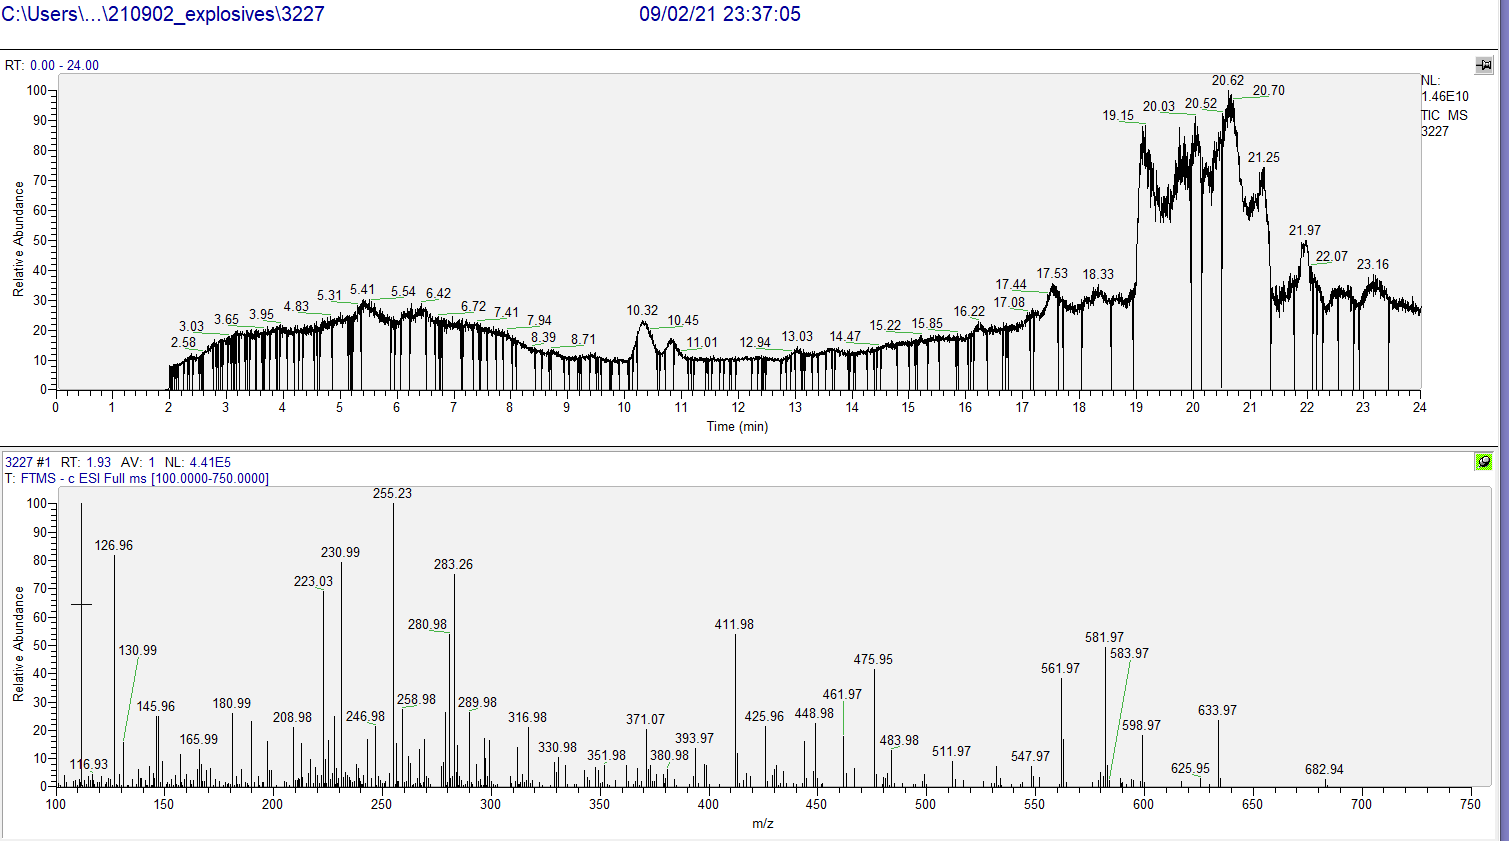
\includegraphics[height=\textheight,%
                   width=\textwidth,%
                   keepaspectratio]{Bilder/TIC_3227_SampleW1.PNG}
\caption{Total Ion Count W01 vom 19.07.2021}
\end{figure}
\begin{figure}[htb]
\includegraphics[height=\textheight,%
                   width=\textwidth,%
                   keepaspectratio]{Bilder/TIC_5ppbSTandard.PNG}
\caption{Total Ion Count - Referenzstandard}
\end{figure}
\begin{figure}[htb]
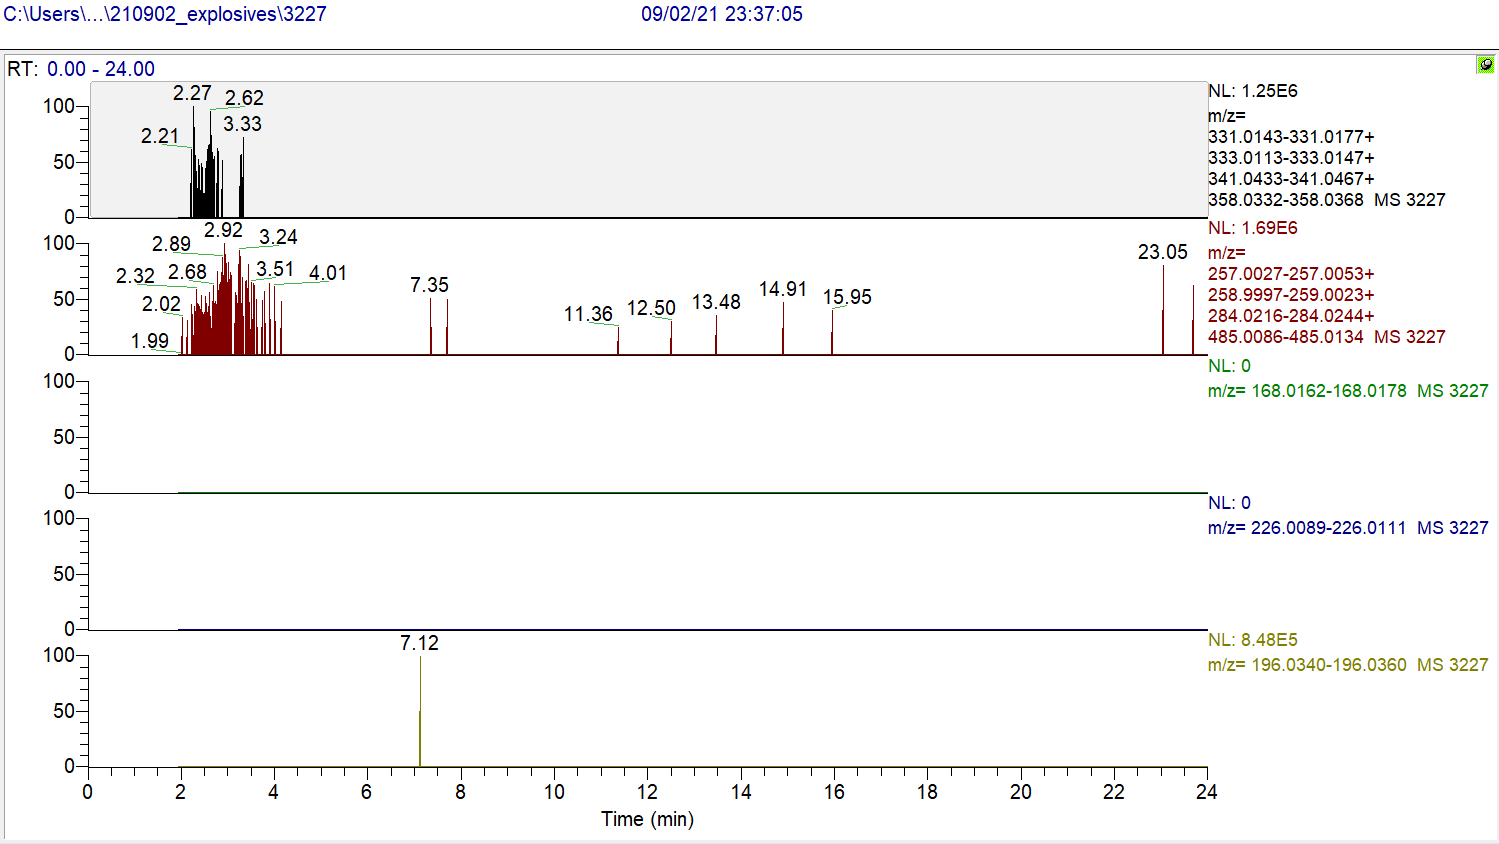
\includegraphics[height=\textheight,%
                   width=\textwidth,%
                   keepaspectratio]{Bilder/Explosives_3227_SampleW1.PNG}
\caption{Chromatografieergebnis mit Focus auf sprengstofftypische Verbindung. Von oben nach unten: HMX (schwarz), RDX (grün), TNT (blau), ADNT (gelb)}
\end{figure}
Es gibt zwei Spitzen für 4-ADNT und 2-ADNT-Isomere.
Was bedeuten die Spitzen bei HMX und RDX?

\begin{figure}[htb]
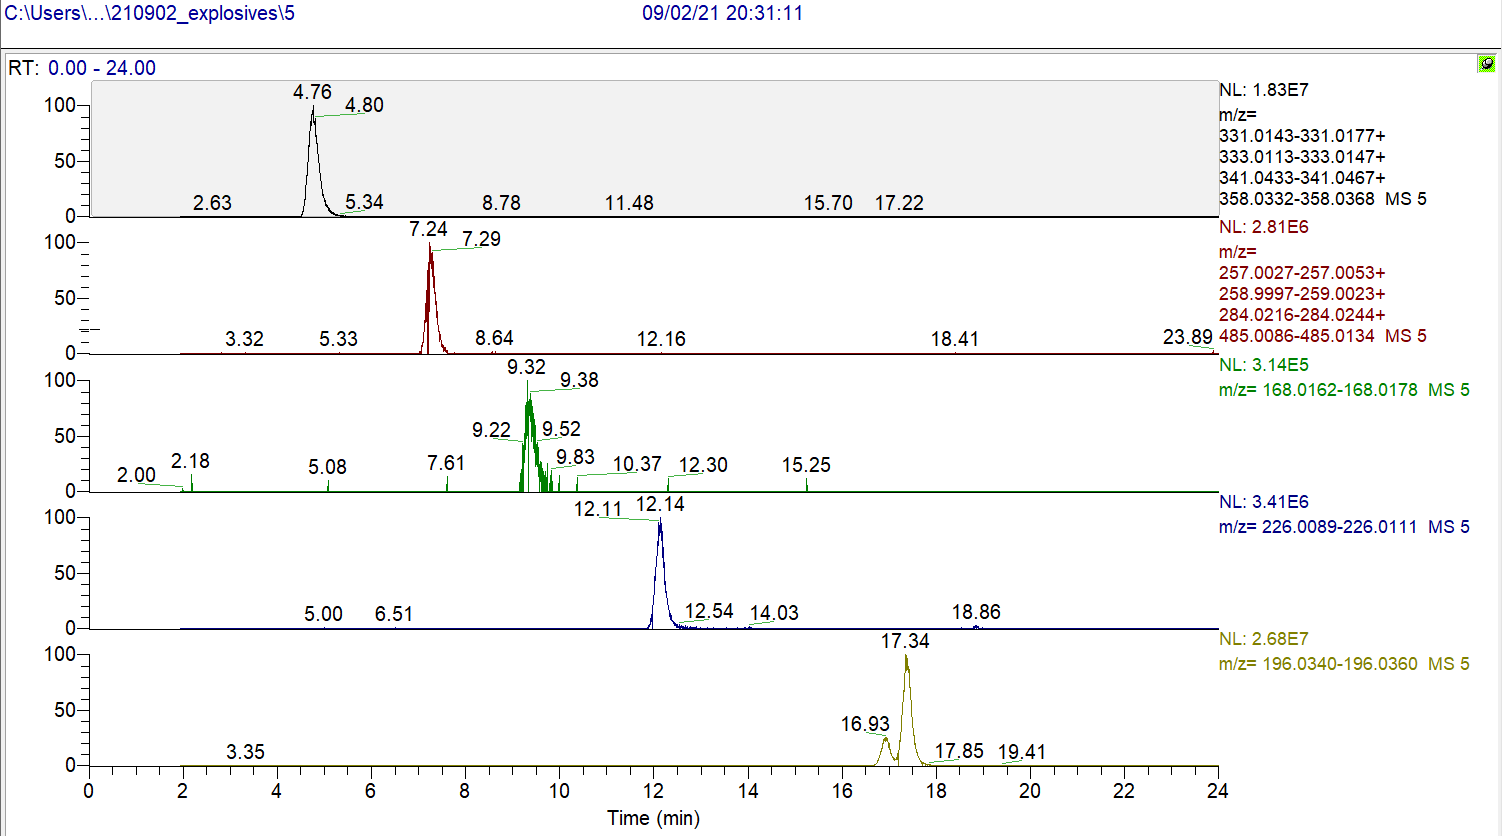
\includegraphics[height=\textheight,%
                   width=\textwidth,%
                   keepaspectratio]{Bilder/Explosives_5ppb.PNG}
\caption{Vergleichende Standardwerte}
\end{figure}
\begin{figure}[htb]
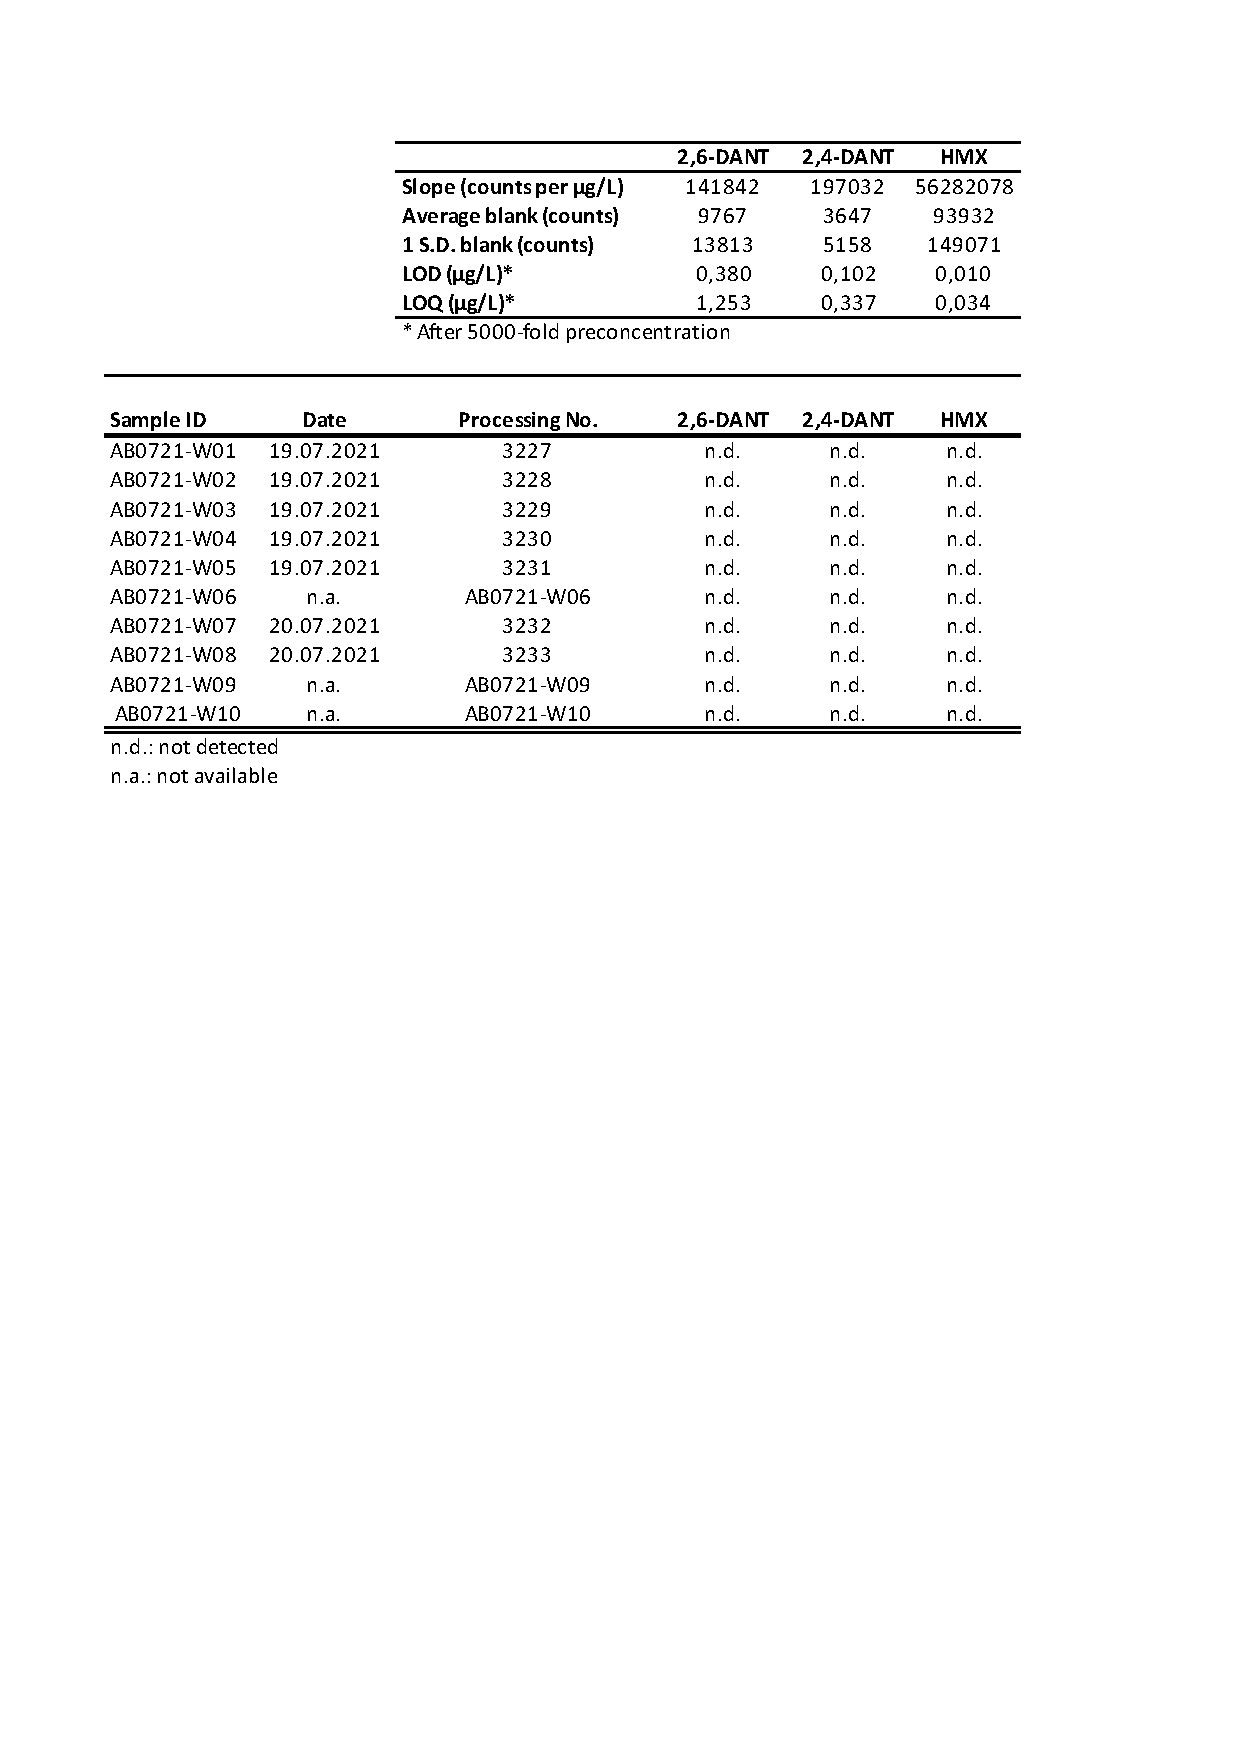
\includegraphics[height=\textheight,%
                   width=\textwidth,%
                   keepaspectratio]{Bilder/MC_data_Aldebaran.pdf}
\caption{Datensatz}
\end{figure}
\section{Diskussion der Ergebnisse}
Wir können Entwarnung geben: Das von uns abgesuchte Gebiet ist unbelastet. Ein
solches Ergebnis ist zwar unspektakulär, jedoch auch erleichternd. Wieso 
unsere Proben keine Spuren von Sprengstoffen oder deren Zerfallsprodukten 
enthalten ist eine andere Frage, möglicherweise wurden sie seit dem xx.xx.xxxx%TODO: DATUM
von der Biomasse vor Ort aufgenommen, und uns bei der Probenfiltrierung
abhanden gekommen. Auf jeden Fall sollten weitere Untersuchungen (vorzugsweise
an Bord der ALDEBARAN) stattfinden, sowie evtl. neue Methoden zur Erfassung
von Sprengstoffen in Organik entwickelt werden.
